%%Tesis
\chapter*{Motivation and Objectives}
\addcontentsline{toc}{chapter}{Motivation and Objectives}
\label{sec:motivation}

In humans, plasma glucose is normally maintained within a narrow range (approximately 65-140 mg/dL), in both the fasting and fed state, due to a tightly linked balance between glucose production (mainly from the liver), absorption (from the gut) and utilization from the muscle, the adipose tissue and the brain. Diabetes Mellitus is a disease characterized by the loss of natural glucose homeostasis, resulting in high glucose concentrations in the patient, which if not treated lead to both chronic (cardiovascular diseases, renal failure or diabetic retinopathy) or acute life-threatening complications (diabetic ketoacidosis and coma).

In the last decades it has become a major health problem worldwide. Its impact all over the world, and especially in the developed countries, has alarmed the health organizations in many countries, and major efforts are being performed to overcome this threat. Scoping into the future is even more shocking. As seen in the report by the IDF of 2013 \cite{IDFatlas}, global diabetes prevalence in 2013 is 8.3\% of the population (382 million people), with a projection in 2035 of 10.1\% prevalence (592 million people). The burden of diabetes is enourmous, causing 5.1 million deaths and taking up about 11\% of the total health spenses in 2013. The increase in population combined with aging of people makes the problem of diabetes to get into epidemic proportions in the next decades, along with a huge economic impact.
%\begin{figure}[hbtp]
%\centering
%\epsfig{file=Figures/diabetes_2010.jpg, width=\textwidth}\caption{Prevalence estimates of diabetes (29-70 years old) in 2010. Extracted from \cite{IDFatlas}}
%\label{fig:diabetes_2010}
%\end{figure}
%\begin{figure}[hbtp]
%\centering
%\epsfig{file=Figures/diabetes_2030.jpg, width=\textwidth}\caption{Prevalence estimates of diabetes (29-70 years old) in 2030. Extracted from \cite{IDFatlas}}
%\label{fig:diabetes_2030}
%\end{figure}
There are two types of diabetes mellitus. Type 1 diabetes mellitus (T1DM) is characterized by absolute insulin deficit due to autoimmune destruction of the pancreatic beta cells, which are the natural insulin providers in a healthy person. This condition requires of exogenous insulin delivery to the patient. On the other hand, type 2 diabetes is caused by two different, but related, alterations: insulin resistance, and impaired beta cell function. Type 2 diabetes results in a relative insulin deficit which can be coped with non-pharmacological measures in the early stages of the disease. However, the natural progression of type 2 diabetes leads to a progressive loss of beta cell function overtime, yielding finally into a condition of absolute insulin deficit which requires of exogenous insulin delivery to the patient.

Survival of patients with T1DM has increased since the discovery of insulin in 1921 by Banting and Best \cite{banting1922internal} (before the patient died in a few months). Following insulin discovery, efforts were done to ease insulin replacement. In practice, insulin-based treatments palliated the high levels of glucose in blood that are present in diabetic patients. However, insulin physiology was still not perfectly replicated, especially considering that natural insulin secretion occurs in the portal vascular system, while exogenous insulin delivery is done in the subcutaneous tissue. This causes artificial delays in the insulin action with respect to the response of a healthy person. To overcome this limitation, faster absorbing insulin analogs were developed, and administered in different doses over the course of the day of the diabetic person, in order to mimic the behavior of the natural secretion of the pancreas. The subcutaneous route is still a sub-optimal delivery place for even the fastest insulin analogs, causing complications such as hypoglycemia in the case of over-insulinization, or high mean glucose registries in the case of repeated under-insulinization. 

Current insulin-based treatments are administered by the patient under physician advice and supervision, requiring of the patient to be educated in several aspects of the treatment, like carbohydrates estimation in the ingested meals or insulin to carbohydrate ratio in the circadian rhythms. Also, glucose monitoring is traditionally performed using Self Monitoring of Blood Glucose (SMBG), where the patient has to regularly (from 1 to 6 or 7 times per day) measure the capillary blood glucose through finger pricking. These practices are often too complicated and stressful for the patients, causing many therapy mistakes in their daily life, ultimately jeopardizing the quality of life of the diabetic people.

Feasibility of an automatic, portable, insulin delivery system is being researched in the late years under the definition of \emph{Artificial Pancreas}. Such a device is possible due to advances in continuous glucose monitoring and continuous insulin delivery by means of subcutaneous insulin pumps. These advances are specially crucial for patients with type 1 diabetes, who lack of an endogenous insulin secretion by their pancreas. 

Continuous Glucose Monitors (CGM) developed in the last decade have made the artificial control of glucose possible, and their development is under constant review by the scientific community. Although the possibilities of CGM are encouraging, it is not a mature technology, and this type of monitors are subject to poor performance, especially during hypoglycemia and in the area outside the calibration region \cite{mazze2009evaluating}. Despite this, it has been shown that CGM significantly improves glycaemic control in adults with type 1 diabetes \cite{bailey2007reduction} \cite{garg2007continuous}, reducing mean glucose over time, glucose variability and exposure to either hyperglycemia and hypoglycemia. %Nevertheless, its benefits are directly related to the frequency of use, which tends to decrease with time, especially in children and adolescents \cite{juvenile2010effectiveness}. 

Undoubtedly, a potential application of CGM is in the artificial pancreas, driving the automatic infusion of insulin in combination with a subcutaneous insulin pump \cite{hirsch2008clinical}. Despite successful results have been reported in the nocturnal period \cite{clarke2009closed,hovorka2010manual}, the large blood glucose (BG) variability following a meal makes postprandial control still an unmet need. Indeed, rapid glucose fluctuations may affect CGM accuracy \cite{rebrin1999subcutaneous}, which is currently a limiting factor for the controller performance. 

CGM measurements are the main and most important technological source of uncertainty in the glucose profile of a diabetic patient. Every sensor is different, but the principles of sensing used by the most used commercial devices are shared, and consequently dynamics in the error signals can be compared, and thus modeled, easing the characterization of other uncertainty sources. Further uncertainty sources in the diabetic glucose profiles can be listed, such as circadian variability, unmeasured hormone influences, illness, physical activity or meal related uncertainties. Many of these perturbations to the endogenous system are difficult to be measured in a controlled environment, and so far impossible to be predicted in a home setup.

One of the main challenges of the artificial pancreas is the lack of reliable models that closely resemble the physiologic behavior of a diabetic patient's glucose. Many models have been presented and tested in literature, and several cases are exposed in the state of the art of this thesis. However, few current models can be described as accurate representations of diabetic patients, and most of them lack of conclusive validation of diabetic patient's data. Variability within the patient's population, and especially intra-patient variability are the most important problems to be found on the modeling endeavor. Variability prevents repeatability of the results, avoiding the validation of most of the models presented with experimental data, even though mathematical and physiologically the models are well supported. This thesis is devoted to overcome these limitations of the diabetic patient's models.

\section*{Objectives}
\label{sec:Objectives}

Four main objectives are pursued in this thesis:

\begin{enumerate}
	\item \textbf{Efficient protocols for patient identification}. The first objective of this thesis is to analyze the current methodologies of gathering data from diabetic patients in order to facilitate the characterization of real patients. Several cases of optimal experiment design in diabetes are already present in literature, and will be reviewed in the state of the art. Data acquisition from living humans is challenging due to ethical and health safety reasons, and this characteristics of the identification are taken into account in the design of optimal experiments for model identification.
	\item \textbf{Representative glucose sensor modeling}. The second objective is to find an accurate model to simulate continuous glucose monitors and the errors associated to these devices. Modeling the error of the CGM in order to simulate the behavior of the sensors is of the greatest importance for the development of successful controllers for the artificial pancreas.
	\item \textbf{Exploration of possibilities of models with uncertainty}. Many possibilities are available for uncertainty characterization (possibilistic approach, bounded response, local identification...). The third objective in this thesis is to search for the most appropriate method for identifying the variability of the glucose of a type 1 diabetic patient, exploring the possibilities of application on different measuring technologies, such as blood glucose reference and CGM.
	\item \textbf{Uncertainty modeling validation}. The last objective of this thesis is to challenge the models and methods designed with real data from diabetic patients. It is intended that the work performed in here will be of practical use for future research in the field. Therefore, experimental application is probably the most important objective for this thesis.
	
\end{enumerate}

\section*{Outline}
\label{sec:Outline}

\begin{figure}[hbtp]
\centering
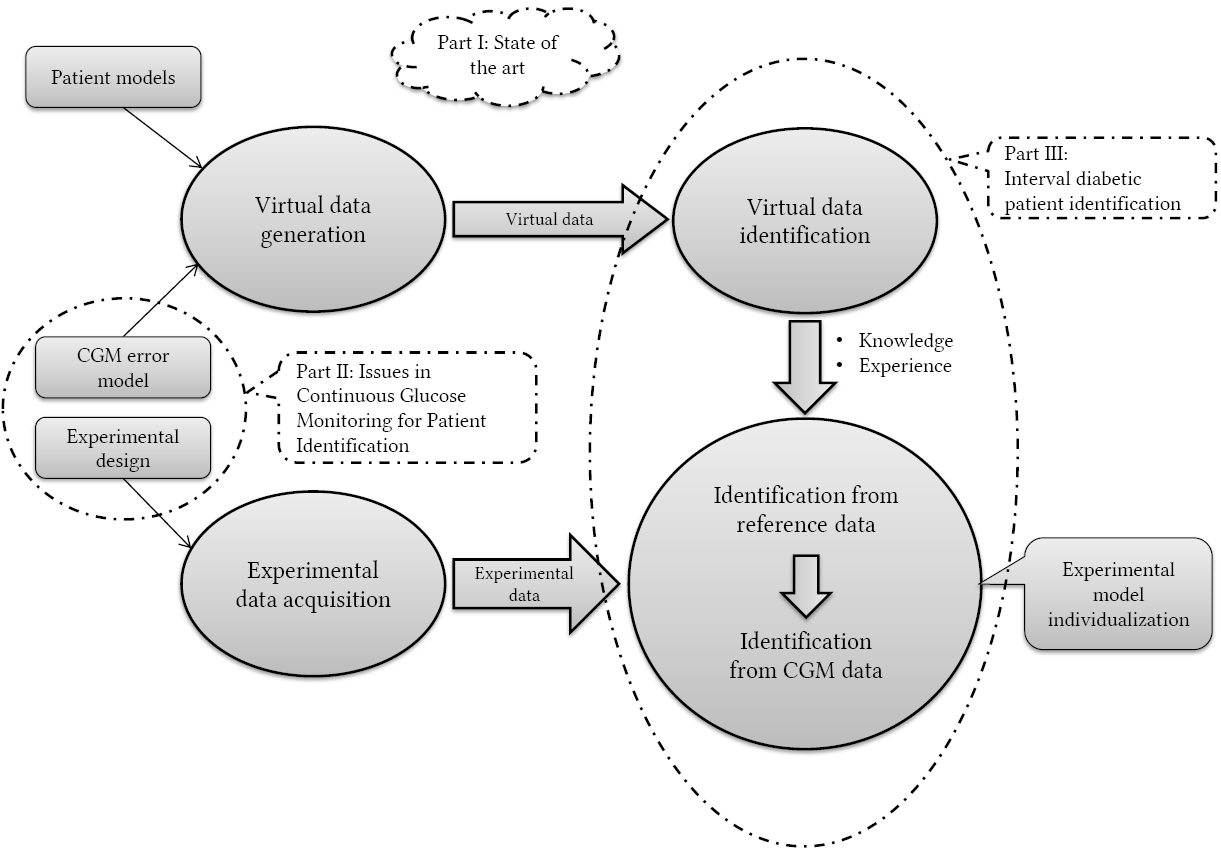
\epsfig{file=Figures/tesis_outline.png, width=\textwidth}\caption{Work-flow schematics for this thesis. The conceptual blocks that correspond to the subsequent parts of this thesis are highlighted in dashed circles.}
\label{fig:thesis_outline}
\end{figure}

A quick visual outline of this thesis contribution can be seen in Figure \ref{fig:thesis_outline}. In there, two work flows can be seen for the execution of an identification experiment in diabetes. This thesis starts (part I) with a literature review of identification in diabetes and associated methodologies. This part of the thesis applies on the background of the workflow depicted in Figure \ref{fig:thesis_outline}.

The first (top) work flow involves the use of virtual patient data for identification experiments. Virtual patient identification is needed for proving the benefits of the proposed identification methodology. The first scientific contributions of this work are comprised in the second part of this thesis, focusing on the improvement of the conditions of identification for both the identification of virtual patients and in the experimental condition. Experimental design focuses on the second (bottom) work flow in Figure \ref{fig:thesis_outline}. This design is carried out using multiple models in order to obtain rich quality data from the diabetic patients. Diabetic patients hospital data is then gathered and analyzed for CGM error modeling, in order to obtain a much more reliable virtual patient simulation, including daily monitoring using a simulated CGM. 

The last part of this thesis is the core identification study. This study is also composed of two parts, one using computer generated data using the CGM models developed earlier, and other using real experimental data from 12 diabetic patients. The differences between virtual and experimental identifications are clearly exposed throughout the thesis, detailing the difficulties that rise when facing real life patient variability. The focus on variability is also constant in this work, and a new identification methodology considering uncertainty is here extensively stated and validated.

\section*{Publications}
\label{sec:Publications}

\subsubsection*{Journal Articles}
\begin{enumerate}
	\item Rossetti P, Ampudia-Blasco F J, Laguna, A J, Revert A, Veh\'{i} J, Ascaso, J F, Bondia J. Evaluation of a Novel Continuous Glucose Monitoring-Based Method for Mealtime Insulin Dosing -the iBolus- in Subjects with Type 1 Diabetes Using Continuous Subcutaneous Insulin Infusion Therapy: A Randomized Controlled Trial. \textit{Diabetes Technology \& Therapeutics} (2012), 14(11), 1043-1052.
  \item Laguna A J, Rossetti P, Ampudia-Blasco F J, Veh\'{i} J, Bondia J. Postprandial performance of Dexcom\textsuperscript{\textregistered} SEVEN\textsuperscript{\textregistered} PLUS and Medtronic\textsuperscript{\textregistered} Paradigm\textsuperscript{\textregistered} Veo\texttrademark{}: Modeling and statistical analysis, \textit{Biomedical Signal Processing \& Control} (2013), http://dx.doi.org/10.1016/j.bspc.2012.12.003
  \item Laguna A J, Rossetti P, Ampudia-Blasco F J, Veh\'{i} J, Bondia J. Identification of intra-patient variability in the postprandial response of patients with type 1 diabetes, \textit{Biomedical Signal Processing \& Control}(2013), http://dx.doi.org/10.1016/j.bspc.2013.07.003
  \item Laguna A J, Rossetti P, Ampudia-Blasco F J, Veh\'{i} J, Bondia J. Experimental blood glucose interval identification of patients with type 1 diabetes, \textit{Journal of Process Control} (2013), 24(1), 171-181.
\end{enumerate}
There is also a paper in preparation with the contents of chapter \ref{sec:ExperimentalIntervalIdentification}.

\subsubsection*{Conference Articles}
\begin{enumerate}
	\item Laguna A J, Rossetti P, Ampudia-Blasco F J, Veh\'{i} J, Bondia J. (2010, September). Optimal design for individual model identification based on ambulatory continuous glucose monitoring in patients with type 1 diabetes. In 2010, UKACC International Conference on Control (pp. 1-6).
	\item Bondia J, Laguna A J, Rossetti P, Ampudia-Blasco F J, Veh\'{i} J. (2011, August). On the Use of Hard/soft Specifications to Deal with Intra-Patient Variability in Postprandial Glucose Control in Type 1 Diabetes. In IFAC World Congress (Vol. 18, No. 1, pp. 8347-8353).
	\item Laguna A J, Rossetti P, Ampudia-Blasco F J, Veh\'{i} J, Bondia J. (2012, August). Identification of intra-patient variability in the postprandial response of patients with type 1 diabetes. In BMS symposium (50, 1-6).
\end{enumerate}

\subsubsection*{Conference abstracts and posters}
\begin{enumerate}
	\item Laguna A J, Rossetti P, Ampudia-Blasco F J, Veh\'{i} J, Bondia J. (2010, October). Improving Postprandial Model Identification Using Ambulatory Data from Type 1 Diabetic Patients. In the Diabetes Technology Meeting 2010
	\item Laguna A J, Rossetti P, Ampudia-Blasco F J, Veh\'{i} J, Bondia J. (2011, February). Designing Optimal Ambulatory Conditions to Improve Prediction Capabilities of Individual Post-prandial Glucose Models. In the 4th International Conference in Advance Technologies \& Treatments for Diabetes 2011
	\item Rossetti P, Ampudia-Blasco F J, Laguna A J, Revert, A, Veh\'{i}, J, Ascaso, J F, Bondia J. (2011, April). C\'alculo del bolus prandial utilizando monitorizaci\'on continua de la glucosa en pacientes con diabetes mellitus tipo 1 tratados con infusi\'on subcut\'anea continua de insulina. In Congreso Nacional de la SED 2011
	\item Rossetti P, Ampudia-Blasco F J, Laguna A J, Revert, A, Veh\'{i}, J, Ascaso, J F, Bondia J. (2011, June). A novel strategy for non-empirical prandial insulin administration in subjects with type 1 diabetes (T1DM) treated with continuous subcutaneous insulin infusion (CSII). In the 71st scientific sessions of ADA 2011
	\item Laguna A J, Rossetti P, Ampudia-Blasco F J, Veh\'{i} J, Bondia J. (2012, February). Postprandial behavior of Dexcom\textsuperscript{\textregistered} SEVEN\textsuperscript{\textregistered} PLUS continuous glucose monitoring system: Statistical analysis and simulation. In the 5th International Conference in Advance Technologies \& Treatments for Diabetes 2012
	\item Rossetti P, Ampudia-Blasco F J, Laguna A J, Revert, A, Veh\'{i}, J, Ascaso, J F, Bondia J. (2012, June). Intra-Subject Variability Makes Prediction of Post-Prandial Glucose Response Difficult in Subjects with Type 1 Diabetes. In the 72nd scientific sessions of ADA 2012
	\item Laguna A J, Rossetti P, Ampudia-Blasco F J, Veh\'{i} J, Bondia J. (2013, February) Uncertainty characterization for the artificial pancreas using interval identification in patients with type 1 diabetes. In the 6th International Conference in Advance Technologies \& Treatments for Diabetes 2013
	\item Laguna A J, Rossetti P, Ampudia-Blasco F J, Veh\'{i} J, Bondia J. (2014, Accepted) Identification of variability in postprandial behavior of patients with type 1 diabetes from insulin pump data. In the 7th International Conference in Advance Technologies \& Treatments for Diabetes 2014
\end{enumerate}


 





